% !TEX encoding = UTF-8 Unicode
\documentclass[a4paper, cs4size, oneside]{article}
\usepackage{ctex}
\usepackage{indentfirst}
\usepackage[english]{babel}
\usepackage{geometry}
\usepackage{graphicx}
\usepackage{enumerate}
\usepackage{url}
\usepackage[colorlinks=true, linkcolor=black]{hyperref}
\usepackage{amsmath,bm}
\usepackage{listings}
\usepackage{subfigure}
\usepackage{titletoc}
\usepackage{titlesec}
\usepackage{booktabs}
\usepackage{multirow}
\usepackage{graphicx}
\immediate\write18{texcount -tex -sum  \jobname.tex > \jobname.wordcount.tex}

\newfontfamily\sectionfont{FandolHei}
\newcommand\thezhsection{\chinese {section}}
%\renewcommand\thesection{第\,\thezhsection\,章}
% section居中
\titleformat{\section}{\centering\Large\bfseries}{第\,\thezhsection\,章}{1em}{}
%\titleformat{\chapter}{\centering\Huge\bfseries\chapterfont}{第\,\thezhchapter\,章}{1em}{}
% 加页码
\pagestyle{plain}

\geometry{left=3.18cm,right=3.18cm,top=2.54cm,bottom=2.54cm}
% \linespread{1.2}
% 行距20磅
\setlength{\baselineskip}{20pt}
% 指定代码加粗关键字
\lstset{
  basicstyle=\ttfamily,
  columns=fullflexible,
%   emph={for, let, if, continue},
%   emphstyle=\bfseries\ttfamily,
  keywords={for, let, if, continue},
  keywordstyle=\textbf
}

% Keywords command
\providecommand{\keywords}[1]
{
  \small	
  \textbf{\textit{Keywords:}} #1
}

%记得页边距缩小,行间距扩大,和加粗
\title{口袋妖怪图鉴数据挖掘和探索 \\
--传说小精灵的预测}
\author{陈镜融 \\ 14307130118@fudan.edu.cn}

\begin{document}
\maketitle

\renewcommand{\abstractname}{摘要}

\begin{abstract}

这篇文章对kaggle数据集:口袋妖怪属性数据进行了分析和挖掘,主要解决根据其余属性预测是否神兽(isLegendary)的问题。本文不会花过多的笔墨介绍口袋妖怪各项属性的统计数据分析,统计的工作在广义上也能归类到数据挖掘工作中,它有助于增加我们对数据宏观层面的理解。但由于其通常结论较为平凡,加之在kaggle网站上已经有许多人对口袋妖怪数据做过各个方面的统计分析,故本文对统计工作将一笔带过,不做过多笔墨介绍。本文亦不会对游戏本身作过多介绍。

\end{abstract}

% \dottedcontents{<section>}[<left>]{<above-code>}
% {<label width>}{<leader width>}
%\dottedcontents{section}[2em]{\bfseries}{3.9em}{1pc}
%\dottedcontents{subsection}[0em]{}{3.3em}{2pc}
%\renewcommand{\contentsname}{\centering 目录}
%\tableofcontents
%\newpage

\section{Introduction}
本文所使用的口袋妖怪数据集\footnote{721 Pokemon with stats and types\url{https://www.kaggle.com/abcsds/pokemon} by Alberto Barradas}包含了721只口袋妖怪的属性值。其中包含的字段在数据集描述\footnote{\url{https://gitee.com/LightSwitch/data_mining_project/tree/master/样例数据集/游戏类/pokemon}}中已经有详细的阐释。而在kaggle上,已经有很多人对该数据集中,口袋妖怪的种类,个体值属性(包括攻击、防御、特攻等)甚至是神兽的预测做了详尽的分析\cite{visofpoketype} \cite{pokeanalysis} \cite{worldofpokemon} \cite{explepoketypes} \cite{predictlegendary}。

\section{Legendary Prediction}
初玩口袋妖怪游戏时,我们对全部口袋妖怪并不了解。但大多数时候,我们却能够对路上遇到的野怪或对战怪兽是否是传说中的小精灵(神兽),做出一个较准的猜测。例如在,当我在初次玩口袋妖怪红宝石386完美时钟版时,这个版本的特点是能够通过单机抓到所有精灵,因此许多神兽甚至在地图上就能直接有分布。例如沙漠里的古拉顿,废弃船超级钓竿钓到的盖欧卡,流星瀑布前5级的梦幻(数据显示其并不是神兽),火焰之路的火焰鸟,斗士之路35级的天空龙,日落山上的超梦和凤王等。当玩家在地图上首次遇到这些神兽时,即使排除所遇怪兽特殊等级,在当前区域较为稀有和剧情发展特殊阶段等特点,玩家却任然能大概率猜测出其是否是神兽。我认为这是一个有趣的现象,因此希望利用口袋妖怪属性数据,实现对一只口袋妖怪是否是神兽的预测。这是我做这件事情的动机。

\begin{figure*}[!htb]
\begin{center}
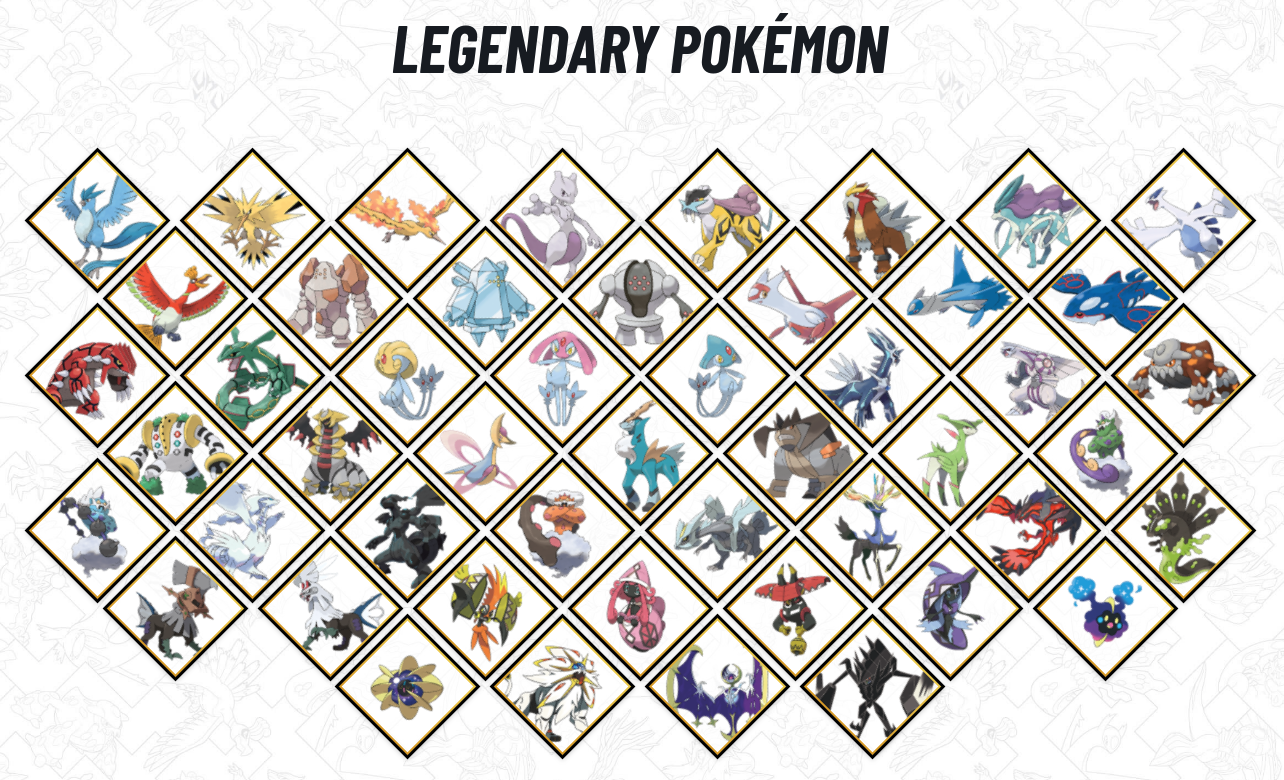
\includegraphics[width=0.7\linewidth]{figures/legendary.png}
\end{center}
   \caption{部分神兽集合}
\label{fig:legendary}
\end{figure*}

\subsection{Naive Boosting Tree}

在这个任务中,观察表格中的属性数据,回顾我作为玩家自身判断未知神奇宝贝是否是神兽的过程,我认为使用决策树这一模型作为分类器更为合适,决策树模型还有利于我们了解判断的过程。

我采用了广为流行的陈天奇大神编写的决策树框架xgboost来进行训练和预测。首先,直观上我们认为口袋妖怪的个体值总和和捕捉率与是否神兽有很强的相关性,神兽往往具有超过580的的个体值,和极低的捕捉率。因此我们首先采用Total和Catch\_Rate两个属性进行决策树的训练。

在划分训练数据和测试数据,我采用前4个世代,共493只宠作为训练数据,剩余第5世代和第6世代的神奇宝贝作为测试样本。训练脚本如下
\begin{lstlisting}
def training(data):
    num_train = 493
    train = data[:num_train, :]
    test = data[num_train:, :]

    train_X = train[:, 1:-1]
    #train_X = normalize(train_X)
    train_Y = train[:, -1]

    test_X = test[:, 1:-1]
    #test_X = normalize(test_X)
    test_Y = test[:, -1]

    xg_train = xgb.DMatrix(train_X, label=train_Y)
    xg_test = xgb.DMatrix(test_X, label=test_Y)

    param = {}
    param['objective'] = 'binary:logistic'
    param['max_depth'] = 3
    param['slient'] = 1
    param['eta'] = 1
    param['nthread'] = 4
    param['eval_metric'] = ['auc', 'ams@0']

    watchlist = [(xg_train, 'train'), (xg_test, 'test')]
    num_round = 5
    bst = xgb.train(param, xg_train, num_round, watchlist)

    pred = np.round(bst.predict(xg_test))
    error_rate = 1.0 * np.sum(pred != test_Y) / test_Y.shape[0]
    print('Test error using logistic = {}'.format(error_rate))

    return bst


def main():
    logger.info('start')
    df = pd.read_csv(config['data_path'], sep=',')
    data_df = pd.DataFrame(
        df, columns=['Name', 'Catch_Rate', 'Total', 'isLegendary'])
    data_df['isLegendary'] = data_df.isLegendary.apply(int)
    data = data_df.values
    model = training(data)
    predict_and_visualize(data, model)
    logger.info('end')

\end{lstlisting}


\begin{figure*}[!htb]
\begin{center}
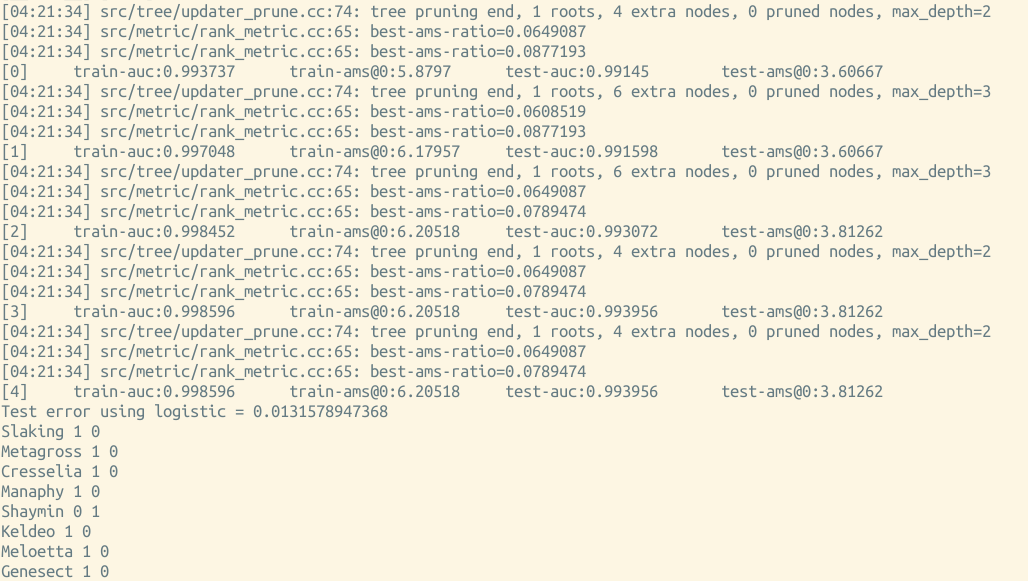
\includegraphics[width=0.7\linewidth]{figures/screenshot1.png}
\end{center}
   \caption{训练输出}
\label{fig:screenshot1}
\end{figure*}

\subsection{Data Correction}

如图\ref{fig:screenshot1}所示,我们可以发现两个事实。第一,仅仅采用个体值总和和捕捉率两个属性,已经可以将神兽判断率达到98\%以上。第二,数据中有错误条目,例如Manaphy和美梦神Cresselia都被归结为非神兽,Mew梦幻,Genesect盖诺赛克特也被归结为非神兽。而美梦神被归为非神兽的同时,噩梦神却被归为神兽。因此很难找到与数据完全一致的神兽划分方法,所以需要对数据进行清洗。由于数据总量较小,因此我采取直接对数据进行修改的方式清洗。神兽数据的标注以这个网址\url{http://nintendo.wikia.com/wiki/Legendary_Pok%C3%A9mon}为标准。我进行修改的宝可梦分别有Mew, Celebi, Cresselia, Manaphy, Keldeo, Meloetta, Genesect.

在对数据进行修正之后,决策树的准确率达到了超过0.99。表\ref{tab:result1}所示是在数据修正过之后,识别错误的所有样例。

\begin{table}[]
\centering
\caption{\textbf{预测错误的例子}}
\label{tab:result1}
\begin{tabular}{ccc}
\hline
\multicolumn{1}{l}{\textbf{}} & \textbf{Predict} & \textbf{Truth} \\ \hline
\textbf{Mew}                  & 0                & 1              \\
\textbf{Celebi}               & 0                & 1              \\
\textbf{Metagross}            & 1                & 0              \\
\textbf{Rayquaza}             & 0                & 1              \\
\textbf{Shaymin}              & 0                & 1              \\
\textbf{Xerneas}              & 0                & 1              \\
\textbf{Yveltal}              & 0                & 1              \\ \hline
\end{tabular}
\end{table}

\subsection{Use Regression Model}

接下来我尝试对结果进行优化,首先如图\ref{fig:side:decistion_tree1}和\ref{fig:side:importance1}所示可以观察到决策树的形态和节点上决策的条件,以及每个决策的权重。图中可以看到当前决策其实非常简单,首先判断属性值,属性值小于567.5的判断为非神兽,而大于等于567.5的宝可梦中,判断捕捉率。这里我们发现,上面是神兽判断成非神兽的,都是因为捕捉率实际大于24。图\ref{fig:side:decision_tree1}中还可以看出,构建的分类树还是过于简单,我们希望结果不仅仅是经过两个判断条件直接决定,而是在多次判断中作周旋。同时,二分类问题一样可以转化为一个回归问题,因此我们采用回归树来优化。
\begin{figure}
\begin{minipage}[htb]{0.5\linewidth}
\centering
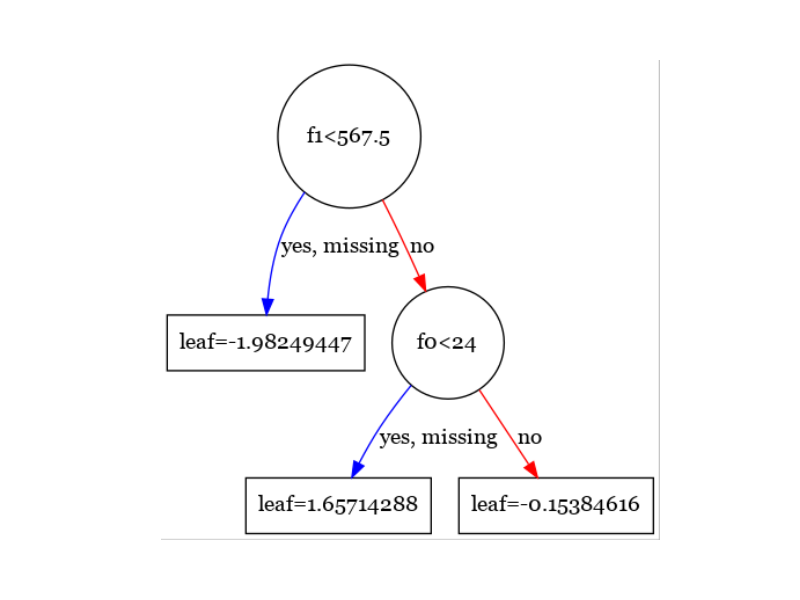
\includegraphics[width=0.9\linewidth]{figures/decision_tree1.png}
\caption{决策树形态}
\label{fig:side:decistion_tree1}
\end{minipage}%
\begin{minipage}[htb]{0.5\linewidth}
\centering
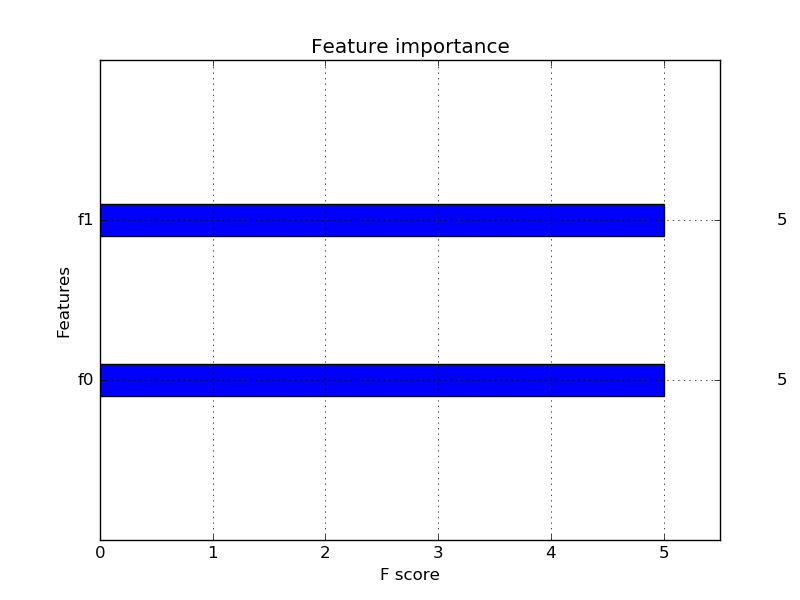
\includegraphics[width=0.9\linewidth]{figures/importance1.png}
\caption{决策权重}
\label{fig:side:importance1}
\end{minipage}
\end{figure}

由图\ref{fig:side:decistion_tree2} \ref{fig:side:importance2}可以看出,采用回归树之后树的形态更加合理,决策权重也有了区分。

\begin{figure}
\begin{minipage}[htb]{0.5\linewidth}
\centering
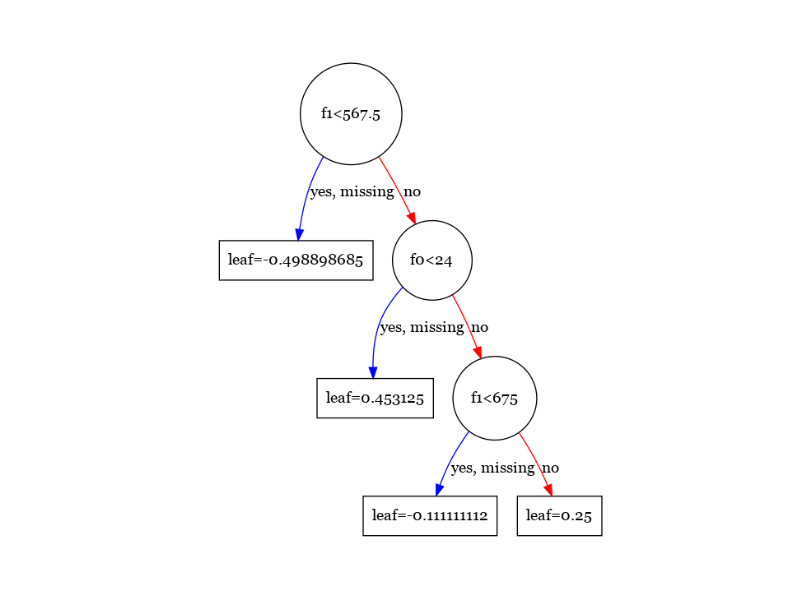
\includegraphics[width=0.9\linewidth]{figures/decision_tree2.png}
\caption{回归决策树形态}
\label{fig:side:decistion_tree2}
\end{minipage}%
\begin{minipage}[htb]{0.5\linewidth}
\centering
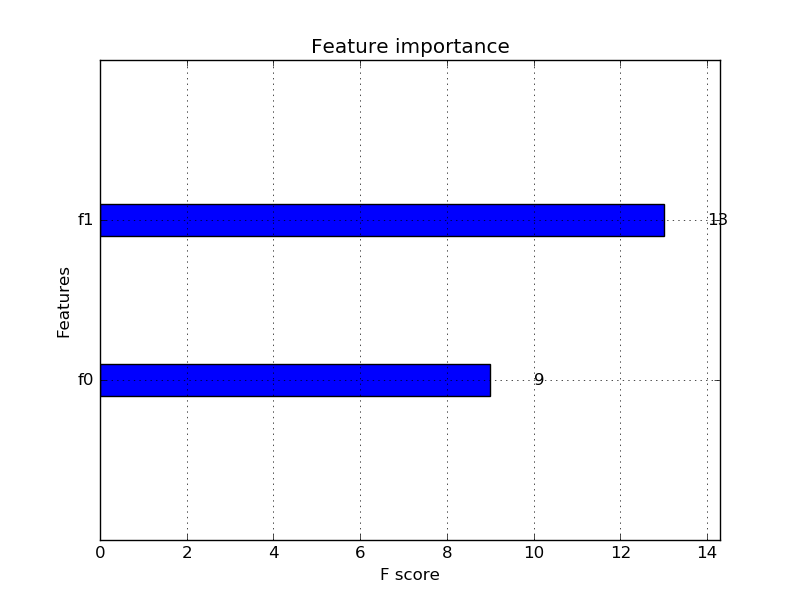
\includegraphics[width=0.9\linewidth]{figures/importance2.png}
\caption{回归树决策权重}
\label{fig:side:importance2}
\end{minipage}
\end{figure}

\begin{table}[]
\centering
\caption{\textbf{采用回归树之后预测错误的例子}}
\label{tab:result2}
\begin{tabular}{cccl}
\hline
\multicolumn{1}{l}{\textbf{}} & \textbf{Predict} & \textbf{Truth} & Predict value \\ \hline
\textbf{Mew}                  & 0                & 1              & 0.4134221     \\
\textbf{Celebi}               & 0                & 1              & 0.4134221     \\
\textbf{Metagross}            & 1                & 0              & 0.90167487    \\
\textbf{Shaymin}              & 0                & 1              & 0.4134221    
\end{tabular}
\end{table}

如表\ref{tab:result2},这次我们在测试集上获得了100\%的准确率,剩下的这几只也属于比较典型的情况,Mew, Celebi, Shaymin都是小个子,在拥有600个体值的情况下,拥有更高一点的捕捉率,而Metagross合金十字也是号称准神兽,同时还和大多数神兽一样没有性别区分,因此更加增加了区分难度。

因此需要进一步采用更多参数来进行优化。

\subsection{Correlation Analysis}

考虑计算属性之间的相关性如表\ref{tab:correlation1},图中将关键的具有较强正相关和负相关的项加粗表示。如图所示,是否神兽这一行,与个体总能力值,是否具有性别,身高,体重和捕捉率都具有一定的相关性。其中,神兽往往具有更强的个体能力值,神兽往往不具有性别区分,神兽的身高和体重往往较大,捕捉率较低。


\begin{table}[]
\centering
\caption{\textbf{各个数值属性之间的相关性}}
\label{tab:correlation1}
\resizebox{\textwidth}{!}{%
\begin{tabular}{l|llllllllllllllll}
\textbf{}        & Number       & Total                 & HP           & Attack       & Defense      & Sp\_Atk      & Sp\_Def      & Speed        & Generation   & isLegendary           & hasGender             & Pr\_Male     & hasMegaEvolution & Height\_m            & Weight\_kg           & Catch\_Rate           \\ \hline
Number           & 1            & 0.160369563           & 0.107512177  & 0.138104374  & 0.121401288  & 0.120160734  & 0.111821733  & 0.028156109  & 0.983328792  & 0.135022334           & -0.100327602          & -0.013413582 & -0.117980945     & -0.009710086         & 0.087309242          & -0.074931499          \\
Total            & 0.160369563  & 1                     & 0.642628024  & 0.704163938  & 0.605831211  & 0.723736779  & 0.706501065  & 0.548890201  & 0.092867967  & \textbf{0.481837163}  & -0.385978146          & 0.113564073  & 0.228502713      & \textbf{0.526813274} & \textbf{0.535965723} & \textbf{-0.738279649} \\
HP               & 0.107512177  & 0.642628024           & 1            & 0.431680156  & 0.228834062  & 0.368639721  & 0.376005602  & 0.17003078   & 0.071545207  & 0.258925937           & -0.155031084          & -0.066703814 & 0.093708108      & 0.442871985          & 0.431319547          & -0.478724989          \\
Attack           & 0.138104374  & 0.704163938           & 0.431680156  & 1            & 0.433232841  & 0.335204871  & 0.207210585  & 0.33501301   & 0.093857362  & 0.302785705           & -0.196892025          & 0.213882027  & 0.203840098      & 0.408589865          & 0.469394833          & -0.525106372          \\
Defense          & 0.121401288  & 0.605831211           & 0.228834062  & 0.433232841  & 1            & 0.20251917   & 0.483986186  & -0.008662735 & 0.068408757  & 0.274446219           & -0.269465674          & 0.06389905   & 0.122665801      & 0.354204998          & 0.47698259           & -0.436557529          \\
Sp\_Atk          & 0.120160734  & 0.723736779           & 0.368639721  & 0.335204871  & 0.20251917   & 1            & 0.492860774  & 0.443106259  & 0.069688917  & 0.409739361           & -0.336579319          & 0.105893343  & 0.175580969      & 0.330579252          & 0.285047951          & -0.539113597          \\
Sp\_Def          & 0.111821733  & 0.706501065           & 0.376005602  & 0.207210585  & 0.483986186  & 0.492860774  & 1            & 0.233487258  & 0.055420507  & 0.360214942           & -0.337264588          & 0.017941206  & 0.149795504      & 0.313195501          & 0.328645452          & -0.513014138          \\
Speed            & 0.028156109  & 0.548890201           & 0.17003078   & 0.33501301   & -0.008662735 & 0.443106259  & 0.233487258  & 1            & 0.003920281  & 0.286082449           & -0.216963966          & 0.070098266  & 0.147844459      & 0.224617151          & 0.108636986          & -0.410557462          \\
Generation       & 0.983328792  & 0.092867967           & 0.071545207  & 0.093857362  & 0.068408757  & 0.069688917  & 0.055420507  & 0.003920281  & 1            & 0.071875318           & -0.029915609          & 0.010911824  & -0.125373799     & -0.051304089         & 0.034002873          & -0.02522699           \\
isLegendary      & 0.135022334  & \textbf{0.481837163}  & 0.258925937  & 0.302785705  & 0.274446219  & 0.409739361  & 0.360214942  & 0.286082449  & 0.071875318  & 1                     & \textbf{-0.644713983} & 0.095427519  & 0.047954911      & 0.32632276           & 0.425219405          & -0.319301622          \\
hasGender        & -0.100327602 & -0.385978146          & -0.155031084 & -0.196892025 & -0.269465674 & -0.336579319 & -0.337264588 & -0.216963966 & -0.029915609 & \textbf{-0.644713983} & 1                     &              & 0.016768986      & -0.200026308         & -0.361465348         & 0.272303615           \\
Pr\_Male         & -0.013413582 & 0.113564073           & -0.066703814 & 0.213882027  & 0.06389905   & 0.105893343  & 0.017941206  & 0.070098266  & 0.010911824  & 0.095427519           &                       & 1            & 0.031730576      & 0.040863021          & 0.061196423          & -0.253644686          \\
hasMegaEvolution & -0.117980945 & 0.228502713           & 0.093708108  & 0.203840098  & 0.122665801  & 0.175580969  & 0.149795504  & 0.147844459  & -0.125373799 & 0.047954911           & 0.016768986           & 0.031730576  & 1                & 0.19462119           & 0.129056546          & -0.173273087          \\
Height\_m        & -0.009710086 & \textbf{0.526813274}  & 0.442871985  & 0.408589865  & 0.354204998  & 0.330579252  & 0.313195501  & 0.224617151  & -0.051304089 & 0.32632276            & -0.200026308          & 0.040863021  & 0.19462119       & 1                    & \textbf{0.661341503} & -0.382862499          \\
Weight\_kg       & 0.087309242  & \textbf{0.535965723}  & 0.431319547  & 0.469394833  & 0.47698259   & 0.285047951  & 0.328645452  & 0.108636986  & 0.034002873  & 0.425219405           & -0.361465348          & 0.061196423  & 0.129056546      & \textbf{0.661341503} & 1                    & -0.367798108          \\
Catch\_Rate      & -0.074931499 & \textbf{-0.738279649} & -0.478724989 & -0.525106372 & -0.436557529 & -0.539113597 & -0.513014138 & -0.410557462 & -0.02522699  & -0.319301622          & 0.272303615           & -0.253644686 & -0.173273087     & -0.382862499         & -0.367798108         & 1                    
\end{tabular}%
}
\end{table}

\subsection{Use More Attributes}

在有了这些分析的基础上,我们再次进行回归树的训练,这次训练中,我将上述和是否神兽具有较强相关性的数据,包括个体值总和,捕捉率,是否具有性别,身高和体重都加入了进来。为了适应更多的属性,我将决策树的深度调整到了5层,训练轮数仍然是5。在经过这次修改之后,模型在训练集和测试集上都获得了100\%的准确率。同时,决策树的形态和各因此重要性如图\ref{fig:side:decistion_tree3}和\ref{fig:side:importance3}所示。图中可以看出,首先对个体值总和与567.5比大小进行区分。对于神兽,我们再判断其是否具有性别,若没有性别,再以捕捉率24为界区分。若有性别,则观察其体重和身高。这样就能获得100\%的预测准确率了。

\begin{figure*}[!htb]
\begin{center}
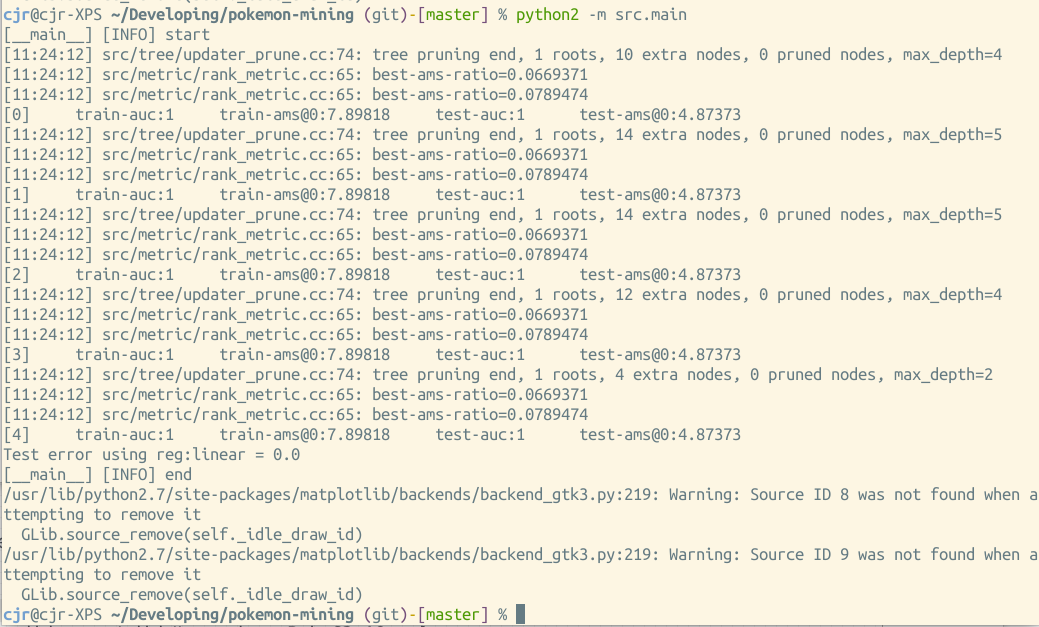
\includegraphics[width=0.7\linewidth]{figures/screenshot3.png}
\end{center}
   \caption{训练输出3}
\label{fig:screenshot3}
\end{figure*}

\begin{figure}
\begin{minipage}[htb]{0.5\linewidth}
\centering
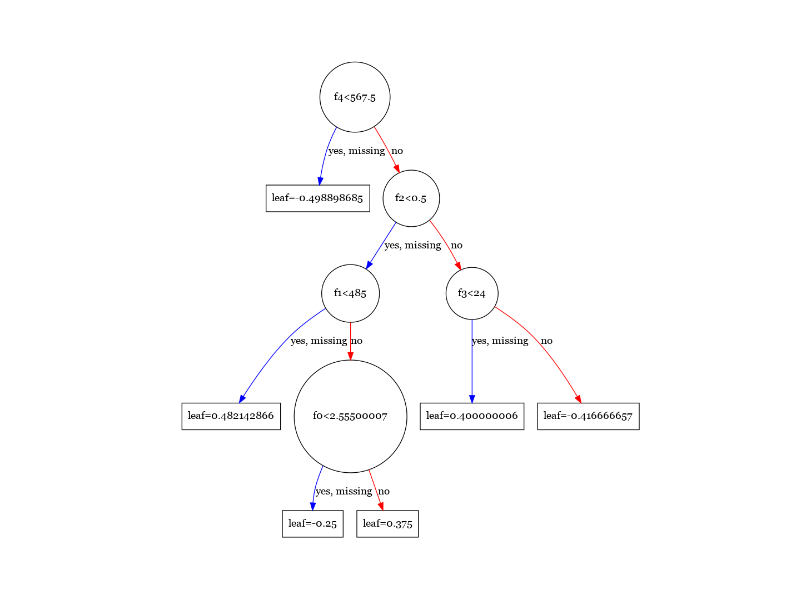
\includegraphics[width=0.9\linewidth]{figures/decision_tree3.png}
\caption{回归决策树形态}
\label{fig:side:decistion_tree3}
\end{minipage}%
\begin{minipage}[htb]{0.5\linewidth}
\centering
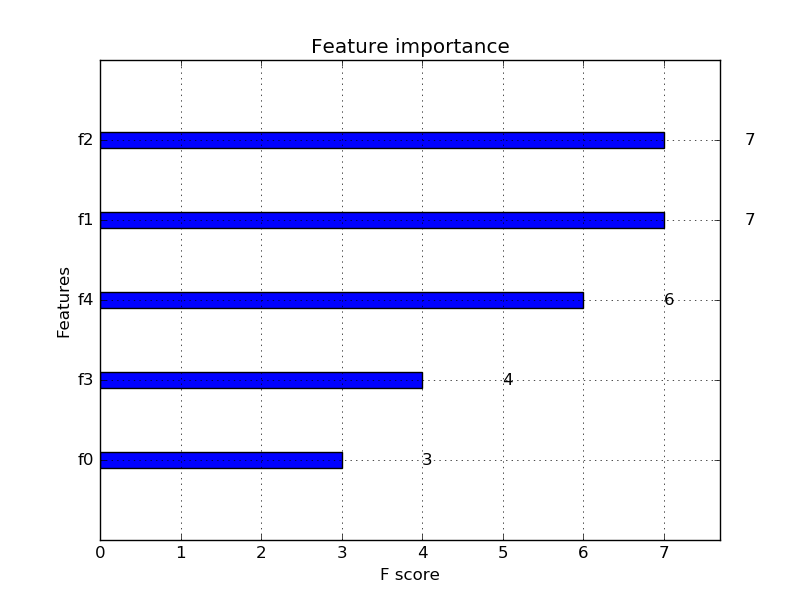
\includegraphics[width=0.9\linewidth]{figures/importance3.png}
\caption{回归树决策权重}
\label{fig:side:importance3}
\end{minipage}
\end{figure}


\section{Conclusion}
总结一下,本文用决策树模型将口袋妖怪数据进行分类和回归训练,进而对一只口袋妖怪是否是神兽进行预测。先后采用了两个属性的简单分类树预测,数据清洗纠正,两个属性的回归树的方法。在对数据属性的相关性做分析之后,加入了更多的关键属性,从而利用5个属性的分类树,最终对神兽预测这个任务达到了100\%的准确率。体验了数据挖掘,分析和优化并验证想法的过程。



\newpage

\addcontentsline{toc}{section}{Reference}

\renewcommand\refname{Reference}
\bibliographystyle{plain}
\bibliography{main}

\clearpage

% Word count
% \verbatiminput{\jobname.wordcount.tex}
\end{document}


%%% 插入图片
% \begin{figure*}[!htb]
% \begin{center}
% \fbox{\rule{0pt}{0in} \rule{0.0\linewidth}{0pt}}
% \includegraphics[width=1.1\linewidth]{图片.png}
% \end{center}
%    \caption{图片标题}
% \label{fig:图形名称}
% \end{figure*}

%%% 插入代码
% \begin{lstlisting}
% type Layer interface {
%     LayerType() LayerType
%     LayerHeader() []byte
%     LayerPayload() []byte
%     // not necessary every Layer can ToBytes, but in our project, it is true
%     ToBytes(data *[]byte) error
% }
% \end{lstlisting}

%%% 将两张图片并排显示
% \begin{figure}
% \begin{minipage}[htb]{0.5\linewidth}
% \centering
% \includegraphics[width=0.9\linewidth]{testcase17.png}
% \caption{测试用例17}
% \label{fig:side:c}
% \end{minipage}%
% \begin{minipage}[htb]{0.5\linewidth}
% \centering
% \includegraphics[width=0.9\linewidth]{testcase19.png}
% \caption{测试用例19}
% \label{fig:side:d}
% \end{minipage}
% \end{figure}
